\subsection{20. Линейные и полулинейные множества. Лемма о том, что для всякого полулинейного множества есть регулярный язык. Теорема Парика: существование КС-языка для полулинейного множества.}

$w \in L: L \subset \Sigma^*$; $\Sigma = \{a_1, a_2, \dots, a_n\}$ $\Rightarrow$ $\exists \psi: \forall w \rightarrow (|w|_{a_1}, |w|_{a_2}, \dots, |w|_{a_n})$

Если $L$ - регулярный язык, то $\psi(L)$ - ?

Введём операции: сложение - $X + Y = \{x + y | x \in X, y \in Y\}$, выпуклая оболочка: $<X> = \{\alpha_1x_1 + \dots + \alpha_nx_n| x_1, \dots, x_n \in X, \alpha_1, \dots, \alpha_n \in \mathbb{Z}^+, \alpha_i \geqslant 0 \}$

$X \subseteq \mathbb{N}^k$, $X = X_1 + <X_2>, |X_1|, |X_2| < \infty$ - \textbf{линейное}

Примеры:

$\psi(abaab) = (3, 2)$; $\psi((ab)^*) = \{(n, n) | n \geqslant 0\}, \psi((ab)^*) = <(1, 1)>$, $\psi((ab)^*) = (0, 0) + <(1, 1)>$ (первая компонента - базовое положение, вторая - разрастание, т.е. идейно это похоже на лемму о разрастании)

$X \subseteq \mathbb{N}^k$ - \textbf{полулинейное}, если X представимо в виде конечного объединения линейных множеств.

Соответственно, язык L - (полу)линейный, если $\psi(L)$ - (полу)линейный.

Утверждение: L - регулярный $\Rightarrow$ L - полулинейный.

\textbf{Лемма:} $\forall X \subseteq \mathbb{N}^{|\Sigma|}$ полулинейного $\exists$ R (полулинейный) - регулярный язык ($\psi(R) = X$)

\textbf{Теорема Па'рика:} L - КС язык $\Rightarrow$ L - полулинейный.

Док-во леммы:

X - полулинейное. Надо найти $R: \psi(R) = X$

$X =X_1 \cup \dots X_l$, $X_i$ - линейное. Для $X_i$ найдём $R_i$: $\psi(R_i) = X_i$; $X_i = \{x_1, \dots, x_m\} + <\{y_1, \dots, y_t\}>$, $x_i, y_i \in \mathbb{N}^{|\Sigma |}$: $x_j \rightarrow u_j: \psi (u_j) = x_j = \{ x_j^1, \dots, x_j^{|\Sigma | } \}$

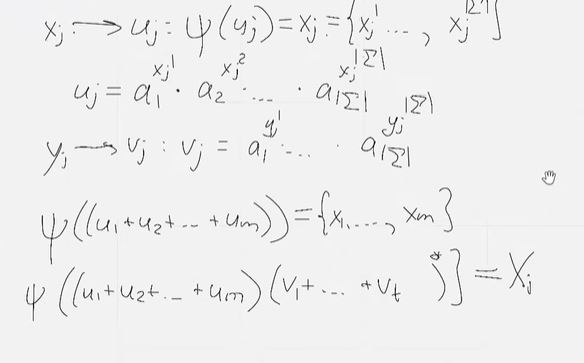
\includegraphics[width=10cm]{images/parikh.JPG}

Нашли для $X_i$, а дальше просто объединение - вот и получили.

